
\begin{figure}[H]
  {
    \setlength{\tabcolsep}{3.0pt}
    \setlength\cmidrulewidth{\heavyrulewidth} % Make cmidrule = 
    \begin{adjustbox}{width=3cm,center}
      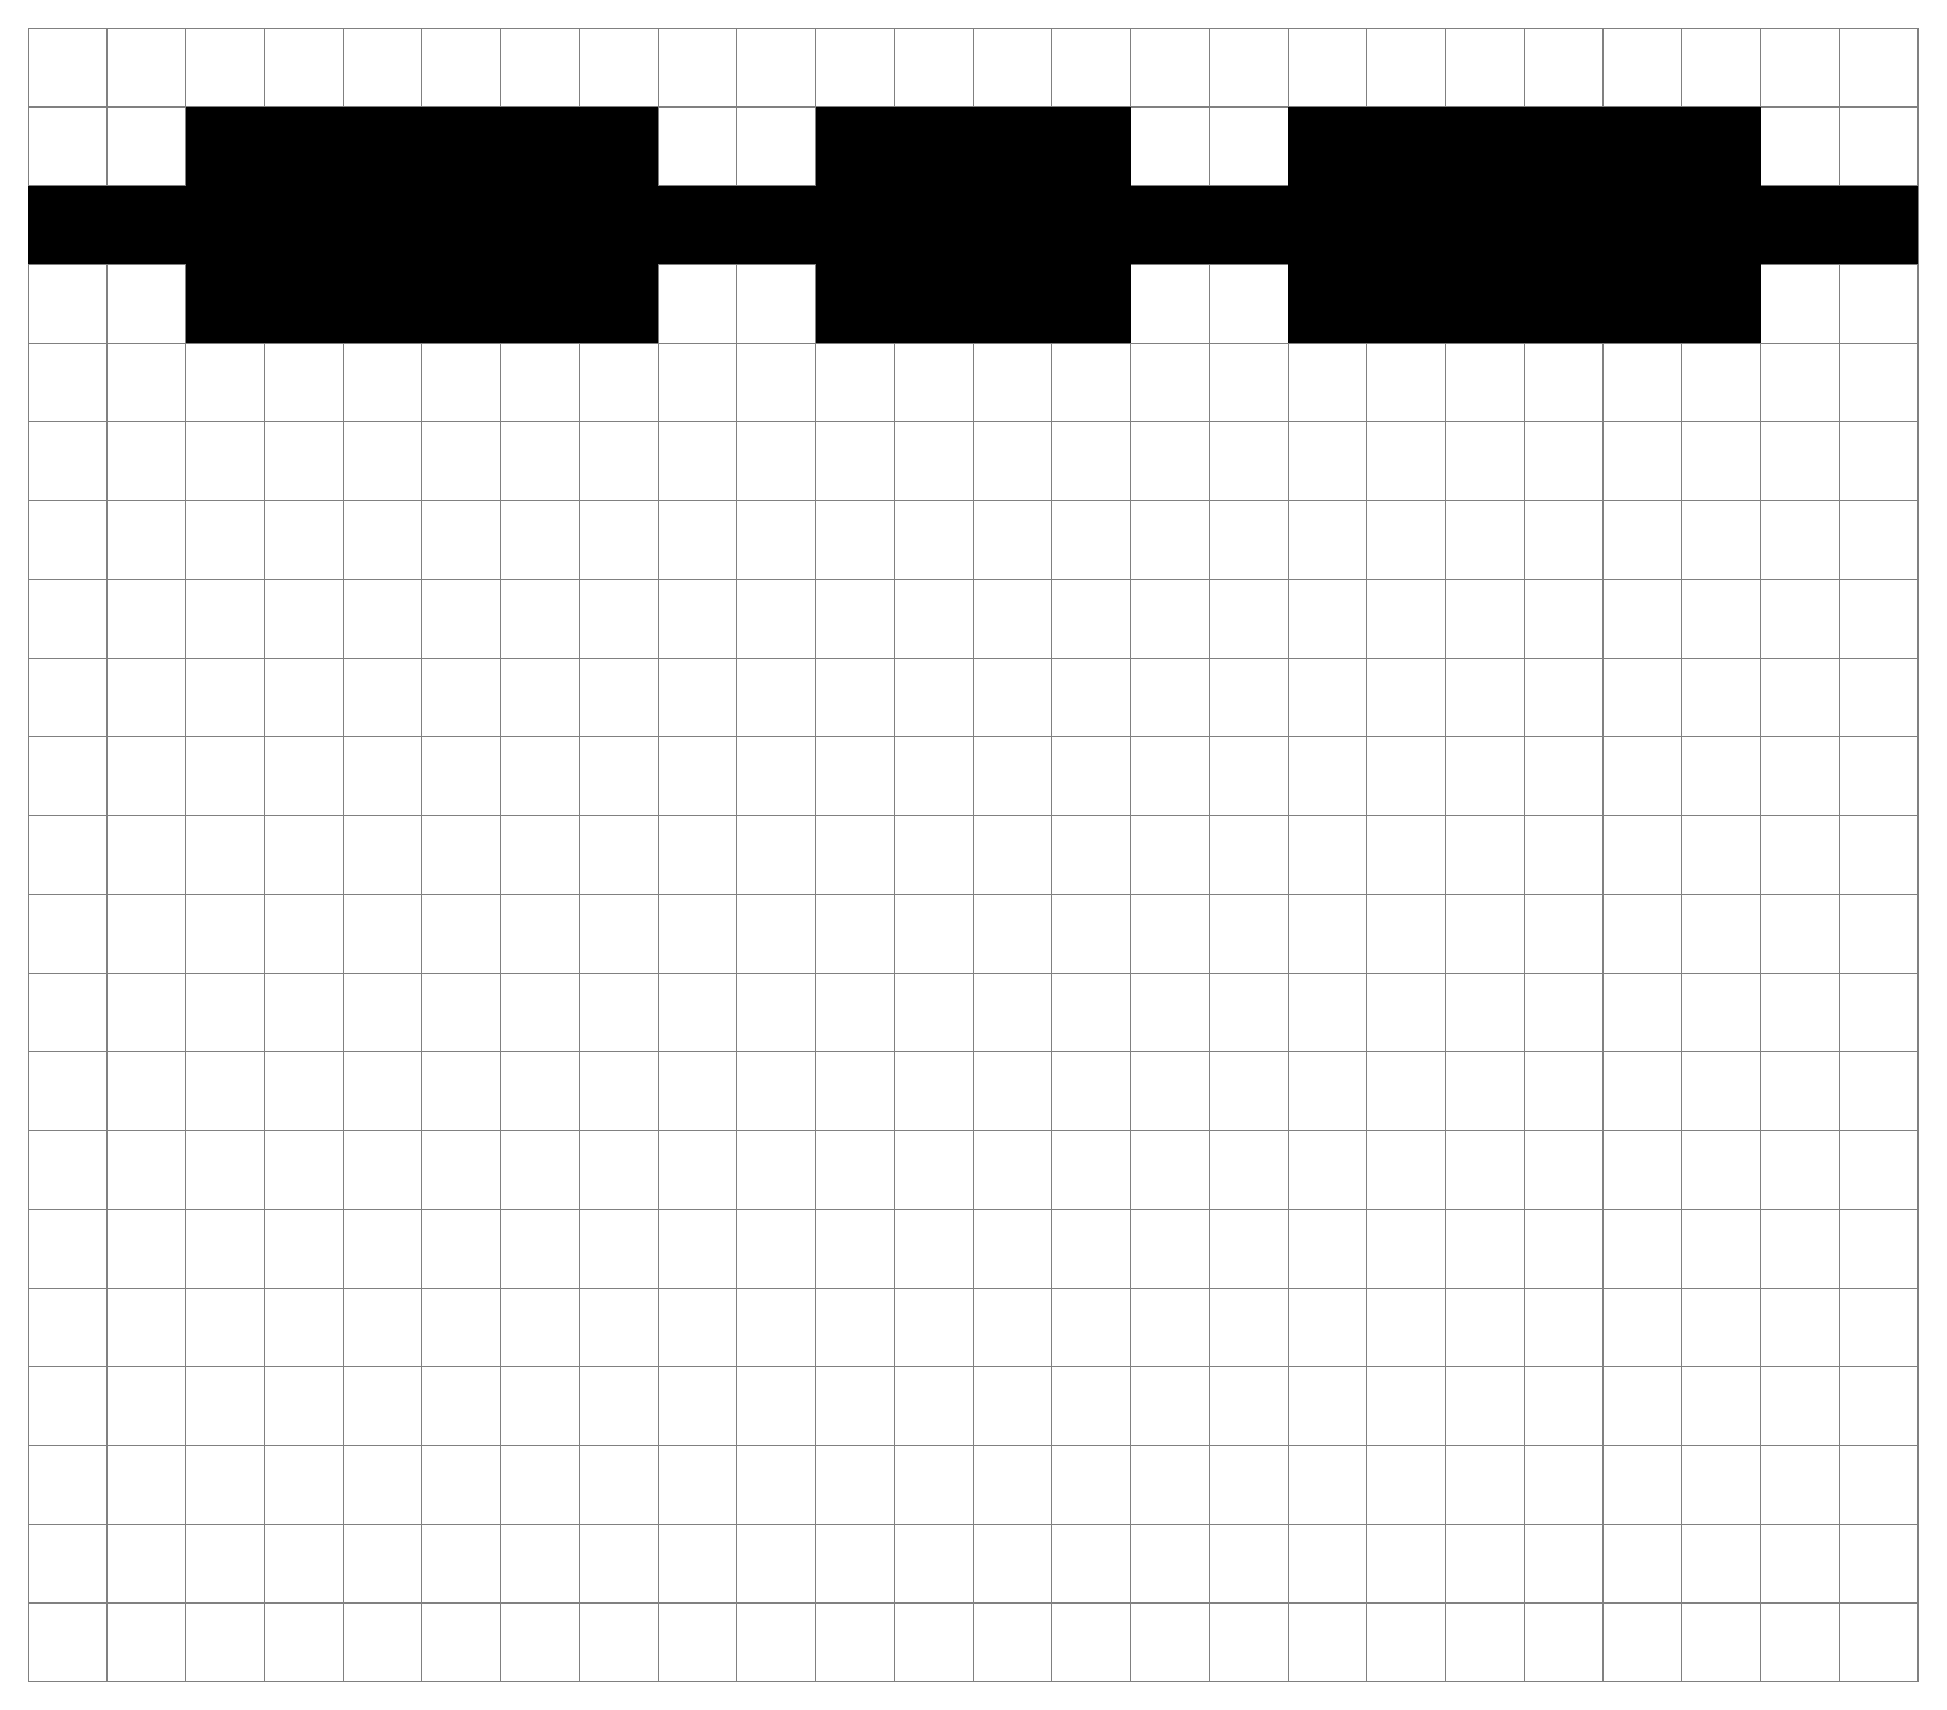
\begin{tikzpicture}

	\draw[step=1.0,gray,thin] (0,0) grid (24,21);
	\fill[\MULTICOLORTWO] (2,19) rectangle ++ (1,1);
	\fill[\MULTICOLORTWO] (3,19) rectangle ++ (1,1);
	\fill[\MULTICOLORONE] (4,19) rectangle ++ (1,1);
	\fill[\MULTICOLORONE] (5,19) rectangle ++ (1,1);
	\fill[\MULTICOLORTWO] (6,19) rectangle ++ (1,1);
	\fill[\MULTICOLORTWO] (7,19) rectangle ++ (1,1);
	\fill[\MULTICOLORONE] (10,19) rectangle ++ (1,1);
	\fill[\MULTICOLORONE] (11,19) rectangle ++ (1,1);
	\fill[\SPRITECOLOR] (12,19) rectangle ++ (1,1);
	\fill[\SPRITECOLOR] (13,19) rectangle ++ (1,1);
	\fill[\MULTICOLORTWO] (16,19) rectangle ++ (1,1);
	\fill[\MULTICOLORTWO] (17,19) rectangle ++ (1,1);
	\fill[\MULTICOLORONE] (18,19) rectangle ++ (1,1);
	\fill[\MULTICOLORONE] (19,19) rectangle ++ (1,1);
	\fill[\MULTICOLORTWO] (20,19) rectangle ++ (1,1);
	\fill[\MULTICOLORTWO] (21,19) rectangle ++ (1,1);
	\fill[\MULTICOLORTWO] (0,18) rectangle ++ (1,1);
	\fill[\MULTICOLORTWO] (1,18) rectangle ++ (1,1);
	\fill[\MULTICOLORTWO] (2,18) rectangle ++ (1,1);
	\fill[\MULTICOLORTWO] (3,18) rectangle ++ (1,1);
	\fill[\MULTICOLORTWO] (4,18) rectangle ++ (1,1);
	\fill[\MULTICOLORTWO] (5,18) rectangle ++ (1,1);
	\fill[\MULTICOLORTWO] (6,18) rectangle ++ (1,1);
	\fill[\MULTICOLORTWO] (7,18) rectangle ++ (1,1);
	\fill[\MULTICOLORTWO] (8,18) rectangle ++ (1,1);
	\fill[\MULTICOLORTWO] (9,18) rectangle ++ (1,1);
	\fill[\MULTICOLORTWO] (10,18) rectangle ++ (1,1);
	\fill[\MULTICOLORTWO] (11,18) rectangle ++ (1,1);
	\fill[\MULTICOLORTWO] (12,18) rectangle ++ (1,1);
	\fill[\MULTICOLORTWO] (13,18) rectangle ++ (1,1);
	\fill[\MULTICOLORTWO] (14,18) rectangle ++ (1,1);
	\fill[\MULTICOLORTWO] (15,18) rectangle ++ (1,1);
	\fill[\MULTICOLORTWO] (16,18) rectangle ++ (1,1);
	\fill[\MULTICOLORTWO] (17,18) rectangle ++ (1,1);
	\fill[\MULTICOLORTWO] (18,18) rectangle ++ (1,1);
	\fill[\MULTICOLORTWO] (19,18) rectangle ++ (1,1);
	\fill[\MULTICOLORTWO] (20,18) rectangle ++ (1,1);
	\fill[\MULTICOLORTWO] (21,18) rectangle ++ (1,1);
	\fill[\MULTICOLORTWO] (22,18) rectangle ++ (1,1);
	\fill[\MULTICOLORTWO] (23,18) rectangle ++ (1,1);
	\fill[\MULTICOLORTWO] (2,17) rectangle ++ (1,1);
	\fill[\MULTICOLORTWO] (3,17) rectangle ++ (1,1);
	\fill[\MULTICOLORONE] (4,17) rectangle ++ (1,1);
	\fill[\MULTICOLORONE] (5,17) rectangle ++ (1,1);
	\fill[\MULTICOLORTWO] (6,17) rectangle ++ (1,1);
	\fill[\MULTICOLORTWO] (7,17) rectangle ++ (1,1);
	\fill[\MULTICOLORONE] (10,17) rectangle ++ (1,1);
	\fill[\MULTICOLORONE] (11,17) rectangle ++ (1,1);
	\fill[\SPRITECOLOR] (12,17) rectangle ++ (1,1);
	\fill[\SPRITECOLOR] (13,17) rectangle ++ (1,1);
	\fill[\MULTICOLORTWO] (16,17) rectangle ++ (1,1);
	\fill[\MULTICOLORTWO] (17,17) rectangle ++ (1,1);
	\fill[\MULTICOLORONE] (18,17) rectangle ++ (1,1);
	\fill[\MULTICOLORONE] (19,17) rectangle ++ (1,1);
	\fill[\MULTICOLORTWO] (20,17) rectangle ++ (1,1);
	\fill[\MULTICOLORTWO] (21,17) rectangle ++ (1,1);

      \end{tikzpicture}
    \end{adjustbox}
  }\caption{LASER\_BULLET}
\end{figure}
